% Chapter 1

\chapter{Introducción general} % Main chapter title

\label{Chapter1} % For referencing the chapter elsewhere, use \ref{Chapter1} 
\label{IntroGeneral}

En el presente capítulo se describen los diferentes métodos de control de acceso en el ámbito de Internet de las Cosas (IoT) y se exponen la motivación, los objetivos y el alcance del trabajo.

%----------------------------------------------------------------------------------------

% Define some commands to keep the formatting separated from the content 
\newcommand{\keyword}[1]{\textbf{#1}}
\newcommand{\tabhead}[1]{\textbf{#1}}
\newcommand{\code}[1]{\texttt{#1}}
\newcommand{\file}[1]{\texttt{\bfseries#1}}
\newcommand{\option}[1]{\texttt{\itshape#1}}
\newcommand{\grados}{$^{\circ}$}

%----------------------------------------------------------------------------------------

%\section{Introducción}

%----------------------------------------------------------------------------------------
\section{Estado del arte}

En esta sección se realiza una introducción a las soluciones IoT y su uso para gestionar el control de acceso en las empresas.

\subsection{Tecnología IoT}

Con la expansión de Internet y las tecnologías de conectividad móvil 3G, 4G y el advenimiento del 5G, se ha producido una revolución en el acceso a la información con un fuerte impacto en la educación, el modo de comunicarnos, las empresas, la ciencia, el gobierno y la humanidad en general. En este contexto, Internet de las Cosas representa la próxima revolución de Internet, dado que su desarrollo está permitiendo dar un gran salto en la capacidad de
reunir, analizar y distribuir datos, convirtiéndolos en información, conocimiento, y en última instancia, sabiduría \citep{WEBSITE:IOT}.

Este término que fue propuesto en 1999, por Kevin Ashton, en el Auto-ID Center del MIT, en donde se realizaban investigaciones sobre RFID y tecnologías de sensores \citep{WEBSITE:IOTMIT}. Es un concepto que refiere a la interconexión digital de objetos cotidianos con Internet \citep{WEBSITE:IOTDefinicion}. Según la definición del Grupo de soluciones empresariales basadas en Internet (IBSG, Internet Business Solutions Group) de Cisco, IoT es sencillamente el punto en el tiempo en el que se conectaron a Internet más ``cosas u objetos'' que personas.

En ese sentido, en 2003 había aproximadamente 6,3 mil millones de personas en el planeta, y 500 millones de dispositivos conectados a Internet. Si dividimos la cantidad de dispositivos conectados por la población mundial de entonces, el resultado era de menos de un dispositivo (0,08) por persona. Mientras que el crecimiento exponencial de los teléfonos inteligentes y las tablets llevó a que en 2010 se elevara a 12,5 mil millones la cantidad de dispositivos conectados a Internet, en tanto la población mundial ascendió a 6,8 mil millones. Tal relación arroja como resultado que el número de dispositivos conectados por persona pasó a ser superior a 1 (1,84 para ser exactos) por primera vez en la historia. En esta línea, se prevé que para el 2025 tendremos alrededor de 41.600 millones de dispositivos conectados \citep{WEBSITE:IOTFechas}.

Conforme lo desarrollado en los párrafos anteriores, IoT se trata principalmente de una red de interconexión digital entre objetos, personas e Internet, que permite el intercambio de datos con otros dispositivos. Esto hace que se pueda capturar información clave sobre el uso y el rendimiento de objetos para así detectar patrones, hacer recomendaciones, mejorar la eficiencia y crear experiencias únicas para los usuarios. En definitiva, esta tecnología está transformando la vida de las personas. Algunos ejemplos son impactantes. Tal es el caso de los pacientes que ingieren dispositivos que
al ingresar a sus cuerpos ayudan a los médicos a diagnosticar y determinar las causas de ciertas enfermedades. También es posible colocar sensores pequeñísimos conectados a Internet en plantas, animales y fenómenos geológicos para medirlos, estudiarlos y prever sus comportamientos. En la figura \ref{fig:Iot} se muestra un diagrama donde se ven las interconexiones de IoT entre dispositivos y los elementos asociados.

\begin{figure}[ht]
	\centering
	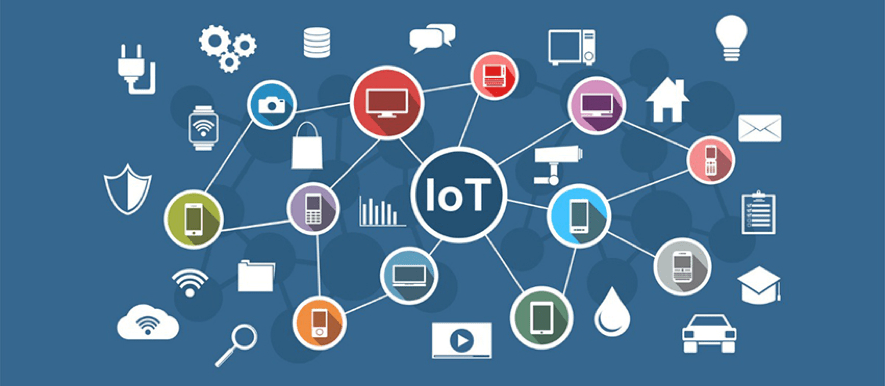
\includegraphics[width=1\textwidth]{./Figures/iot.png}
	\caption{Interconexión de dispositivos y tecnologías en IoT.}
	\label{fig:Iot}
\end{figure}

Resulta importante destacar que existe una correlación directa entre los datos y la sabiduría. Cuántos más datos se generan, más conocimiento y sabiduría pueden obtener las personas. IoT aumenta drásticamente la cantidad de datos que están disponibles para que los procesemos. Este aumento, combinado con la capacidad de Internet de comunicarlos, hará posible que las personas acumulen saberes valiosos. En la figura \ref{fig:Sabiduria} se muestra un diagrama de la correlación entre datos y sabiduría.

\begin{figure}[ht]
	\centering
	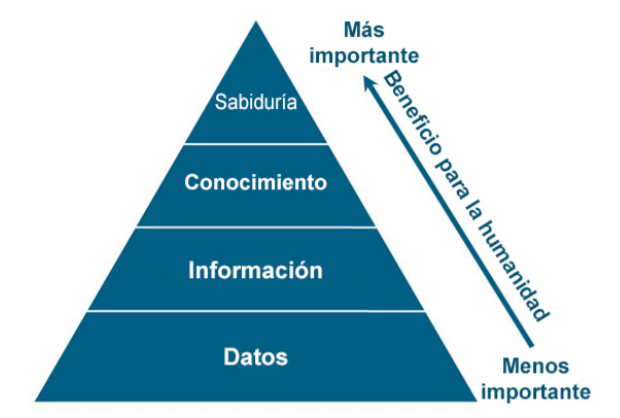
\includegraphics[width=1\textwidth]{./Figures/sabiduria.png}
	\caption{Correlación entre datos y sabiduría.}
	\label{fig:Sabiduria}
\end{figure}

En lo que respecta a las empresas, con el surgimiento de IoT aparece el fenómeno de la transformación digital, que consiste en la aplicación de la tecnología digital para generar un entorno adecuado que facilite la innovación de las empresas y la industria. En este contexto, el desarrollo de nuestro trabajo propone realizar una transformación digital en la empresa Tenaris Metalmecánica, aprovechando estas tecnologías disruptivas.

\subsection{Control de acceso}

El control de acceso se refiere a los mecanismos que permiten o restringen la entrada de una persona o vehículo a una empresa o recinto, mediante su identificación. Dentro de los principales objetivos del control de acceso se incluye el de garantizar la seguridad y facilitar la organización empresarial. Cuando una organización instala un sistema de control de acceso, lo hace básicamente pensando en tres propósitos:

\begin{itemize}
\item Cuidar de la integridad física de las personas.
\item Proteger la información de la compañía (bases de datos, material sensible, etc.).
\item Custodiar los activos de la empresa.
\end{itemize}

Para cumplir con tales propósitos, se emplean diferentes medios para monitorear y controlar el acceso de las personas a una instalación. Décadas atrás se usaban sistemas de cerraduras y llaves. Dicho método, además de ser vulnerable, representaba gastos adicionales para la empresa ante el robo o extravío. Con el advenimiento de Internet, y principalmente de IoT, el control de acceso migró a sistemas más robustos con credenciales electrónicas o identificación biométrica.

\subsubsection{Factores de autenticación}
Para un proceso de identificación, sea físico o digital, se debe comprobar la identidad de la persona que hace la solicitud. Esa verificación se puede realizar usando uno o varios factores de autenticación. Los factores de autenticación se pueden dividir en:

\begin{itemize}
\item Lo que sé: el conocimiento que la persona tiene, puede ser un PIN, una contraseña o un patrón.
\item Lo que tengo: la identificación que posee un individuo para certificar que es él, como una credencial física o virtual.
\item Lo que soy: los rasgos corporales únicos de la persona que se utilizan para verificar la identidad (biometría).
\end{itemize}

Para aumentar el nivel de seguridad, los sistemas modernos implementan varios factores de autenticación en los puntos de acceso, combinando ``lo que tengo'' con ``lo que sé'' y con ``lo que soy'' \citep{WEBSITE:ControlAcceso}.

\subsubsection{Clasificación de sistemas de control de acceso}

Los sistemas de control de acceso para personas se clasifican por dos criterios: conectividad y método de identificación \citep{WEBSITE:ControlAccesoPersonas}.

Por su conectividad:

\begin{itemize}
\item Controles de acceso autónomos: no necesitan conectarse a la red y no guardan datos de los movimientos que producen, sino que se limitan a abrir las puertas o barreras. 
\item Controles de acceso conectados en red: éstos, además de permitir los accesos, registran las entradas y salidas de personas. Deben conectarse a Internet, ya que la información sobre tales movimientos se descarga en una aplicación para poder generar informes.
\end{itemize}

Por su método de identificación:

\begin{itemize}
\item Biométricos: La identificación se produce mediante la lectura de datos físicos individuales que imposibilitan la suplantación al ser intransferibles, por lo que se consideran los sistemas más seguros. Su empleo implica el cumplimiento de normativas en materia de protección de datos y no están permitidos en todas las empresas. Dentro de este grupo tenemos los métodos de reconocimiento facial y huella dactilar.
\item Tarjetas: En muchas oficinas y en otros lugares de trabajo como laboratorios, talleres o fábricas, donde se realizan tareas manuales y por cuestiones de higiene, no se aconseja utilizar la huella dactilar y se emplean, en cambio, llaveros y tarjetas. Estas últimas son de dos clases:
	\begin{itemize}
	\item Tarjetas magnéticas: tienen una banda magnética que contiene los datos de cada persona y se introduce en el lector para solicitar el acceso.
	\item Tarjetas (RFID): utilizan radiofrecuencia y no requieren contacto con el lector para activar el mecanismo que abre la cerradura. Por tal motivo se llaman ``tarjetas de proximidad''.
	\end{itemize}
\item Contraseña numérica: algunos sistemas de control de accesos permiten fichar poniendo una contraseña en el teclado del propio terminal.
\end{itemize}

\subsubsection{Estudio de mercado}

Para nuestro trabajo se realizó un análisis de los sistemas existentes en el mercado y se encontró que la seguridad y confiabilidad de las soluciones existentes van en relación a su precio. Se detectó que la gran mayoría de los sistemas del mercado son cerrados y auto-gestionados, lo que limita su integración con otros sistemas. Dicha limitación atenta contra el valor agregado propuesto en este proyecto.

Por otro lado, si bien existen productos que pueden integrarse con asistentes de voz, como Echo o Alexa de Amazon o Home de Google, en nuestro caso se desaconseja su uso, puesto que éstos recolectan datos sensibles que atentan contra la política de privacidad empresarial. También hay sistemas que permiten el acceso mediante huella, lo cual puede resultar muy cómodo, pero no es útil en la locación industrial donde se va a implementar el trabajo, ya que se requiere una política especial para el guardado de los datos y no divulgación de las huellas dactilares. 

En el capítulo 4, en la sección \ref{sec:comparativa} se realiza un análisis comparativo de las soluciones estudiadas y las ventajas y desventajas en relación con el trabajo desarrollado. En particular se analizaron dos soluciones, una de Pronext (Pronext KY800 \citep{WEBSITE:Ponext}) y una de Samsung (Samsung SHS-H505 \citep{WEBSITE:Samsung}). Si bien dichas soluciones no son costosas y brindan algunas características interesantes como doble factor de autenticación
o acceso mediante huella, no soportan conexión con sistemas externos. Dicha situación no permite el agregado de valor a los datos recolectados y su trasformación en información valiosa para la toma de decisiones.


%----------------------------------------------------------------------------------------

\section{Motivación}

La empresa Tenaris Metalmecánica cuenta con una planta industrial que elabora varillas de bombeo para la extracción de petróleo. Para ello, en sus procesos productivos utiliza servicios de terceros a fin de implementar mejoras en éstos y realizar obras civiles y mecánicas. Todo personal externo que ingresa a la planta debe cumplir un conjunto de requisitos legales y médicos. De este modo, si sucede algún incidente o accidente, la empresa está cubierta y evita problemas legales. Durante el último año se detectaron en auditorías internas varios eventos de ingresos de usuarios con documentación vencida. Por lo tanto, se necesita actuar con celeridad e implementar un sistema de control que detecte y bloquee estos accesos indebidos.

Adicionalmente, ante la necesidad de mejorar la calidad de los productos manufacturados a clientes, se requiere contar con alertas tempranas ante desvíos en los diferentes procesos industriales y de soporte de la empresa. En tal sentido, se han identificado problemas recurrentes que son planteados en reuniones diarias de gestión, pero que quedan sin solución por no ser abordados sistemáticamente. Estas dificultades han derivado en no conformidades de calidad, pérdida de dinero para la empresa y tiempo de recursos humanos valiosos. Por lo tanto, se requiere generar, conjuntamente al sistema de control de terceros, un sistema integral de gestión de alertas que permita activar diferentes tipos de actuadores y adaptarse a distintos casos de uso que se irán agregando en sucesivas etapas. 

En esta primera instancia y para el trabajo proyectado, el objetivo será controlar los ingresos de terceros a la planta y sentar las bases para poder implementar a futuro el sistema de gestión integral mencionado.

%----------------------------------------------------------------------------------------

\section{Objetivos y alcance}

De acuerdo a lo expuesto anteriormente, el alcance de este proyecto incluye el desarrollo de una plataforma de software y módulos de actuación y sensado para el control de ingreso de terceros a planta. A su vez, la plataforma deberá quedar preparada para la incorporación futura de nuevos módulos de sensado y actuación, de modo que solo sea necesario desarrollarlos y configurarlos para que queden acoplados a la misma.

Dentro de la plataforma de software se implementarán los servicios necesarios para la recepción de alarmas mediante \textit{web services} y se generarán la infraestructura y las estructuras de datos necesarias para modelizar alertas, tareas y actuadores genéricos. 

Adicionalmente, se desarrollará un módulo de sensado para leer tarjetas RFID que se asignarán a cada tercero que quiera ingresar a planta. Por último, se prevé la incorporación de un módulo de actuación para liberar o bloquear la cerradura de entrada a la planta, junto a una alarma visual que indique la habilitación o no del usuario. Ambos módulos serán componentes electrónicos o controladores que se encargarán del sensado o actuación y la comunicación de estos sensores y actuadores con la plataforma de software, ya sea mediante una red cableada o Wi-Fi, según la disponibilidad de infraestructura. La plataforma de software se implementará dentro de la Intranet de la empresa en la arquitectura existente.

No se incluirán los módulos para la configuración automática de las tareas, alertas y actuadores por parte del usuario. Tampoco se agregarán módulos de sensado o actuación adicionales.

A los fines de determinar si un usuario está habilitado o no para ingresar a planta se consultará con un sistema de documentación de terceros que ya está operativo en la empresa. El mismo permite conocer si el tercero está activo (está prestando servicios actualmente en la empresa o fue dado de baja por fin de su contratación) y si tiene toda la documentación requerida al día. Nuestro desarrollo se comunicará con éste a través de la Intranet de la empresa.

En la figura \ref{fig:Solucionbasica} se muestra el diagrama en bloques de la solución y sus interfaces.

\begin{figure}[th]
	\centering
	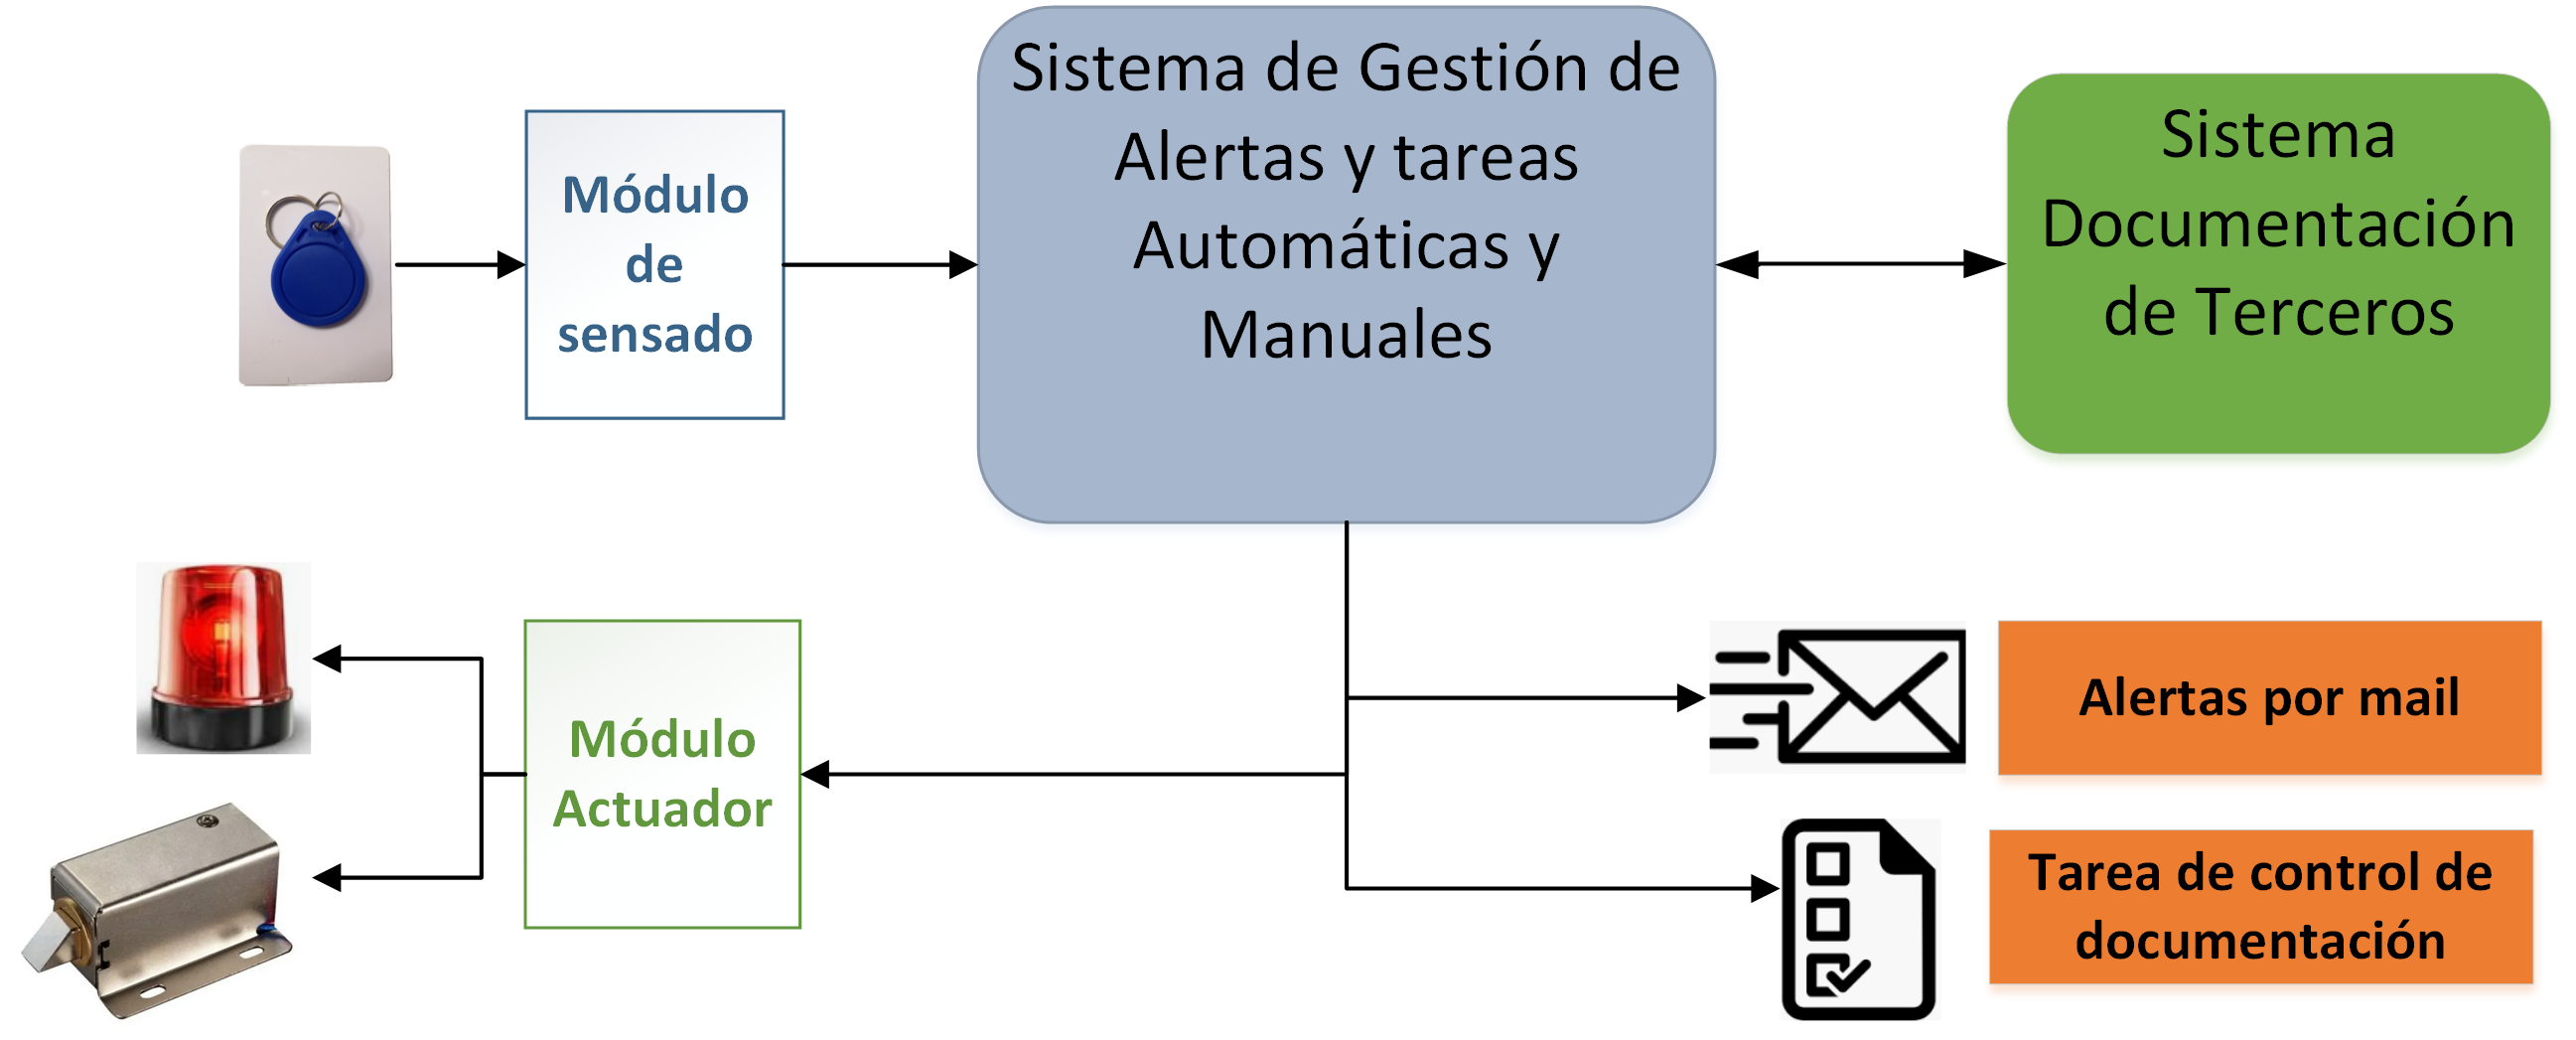
\includegraphics[width=1\textwidth]{./Figures/solucionbasica.png}
	\caption{Diagrama en bloques de la solución propuesta.}
	\label{fig:Solucionbasica}
\end{figure}


%----------------------------------------------------------------------------------------

